\chapter{The Cassini-Huygens Mission}
\label{chap:cassini}
\section{Overview}
%http://sci.esa.int/cassini-huygens/33415-summary/
\begin{figure}
\centering
\noindent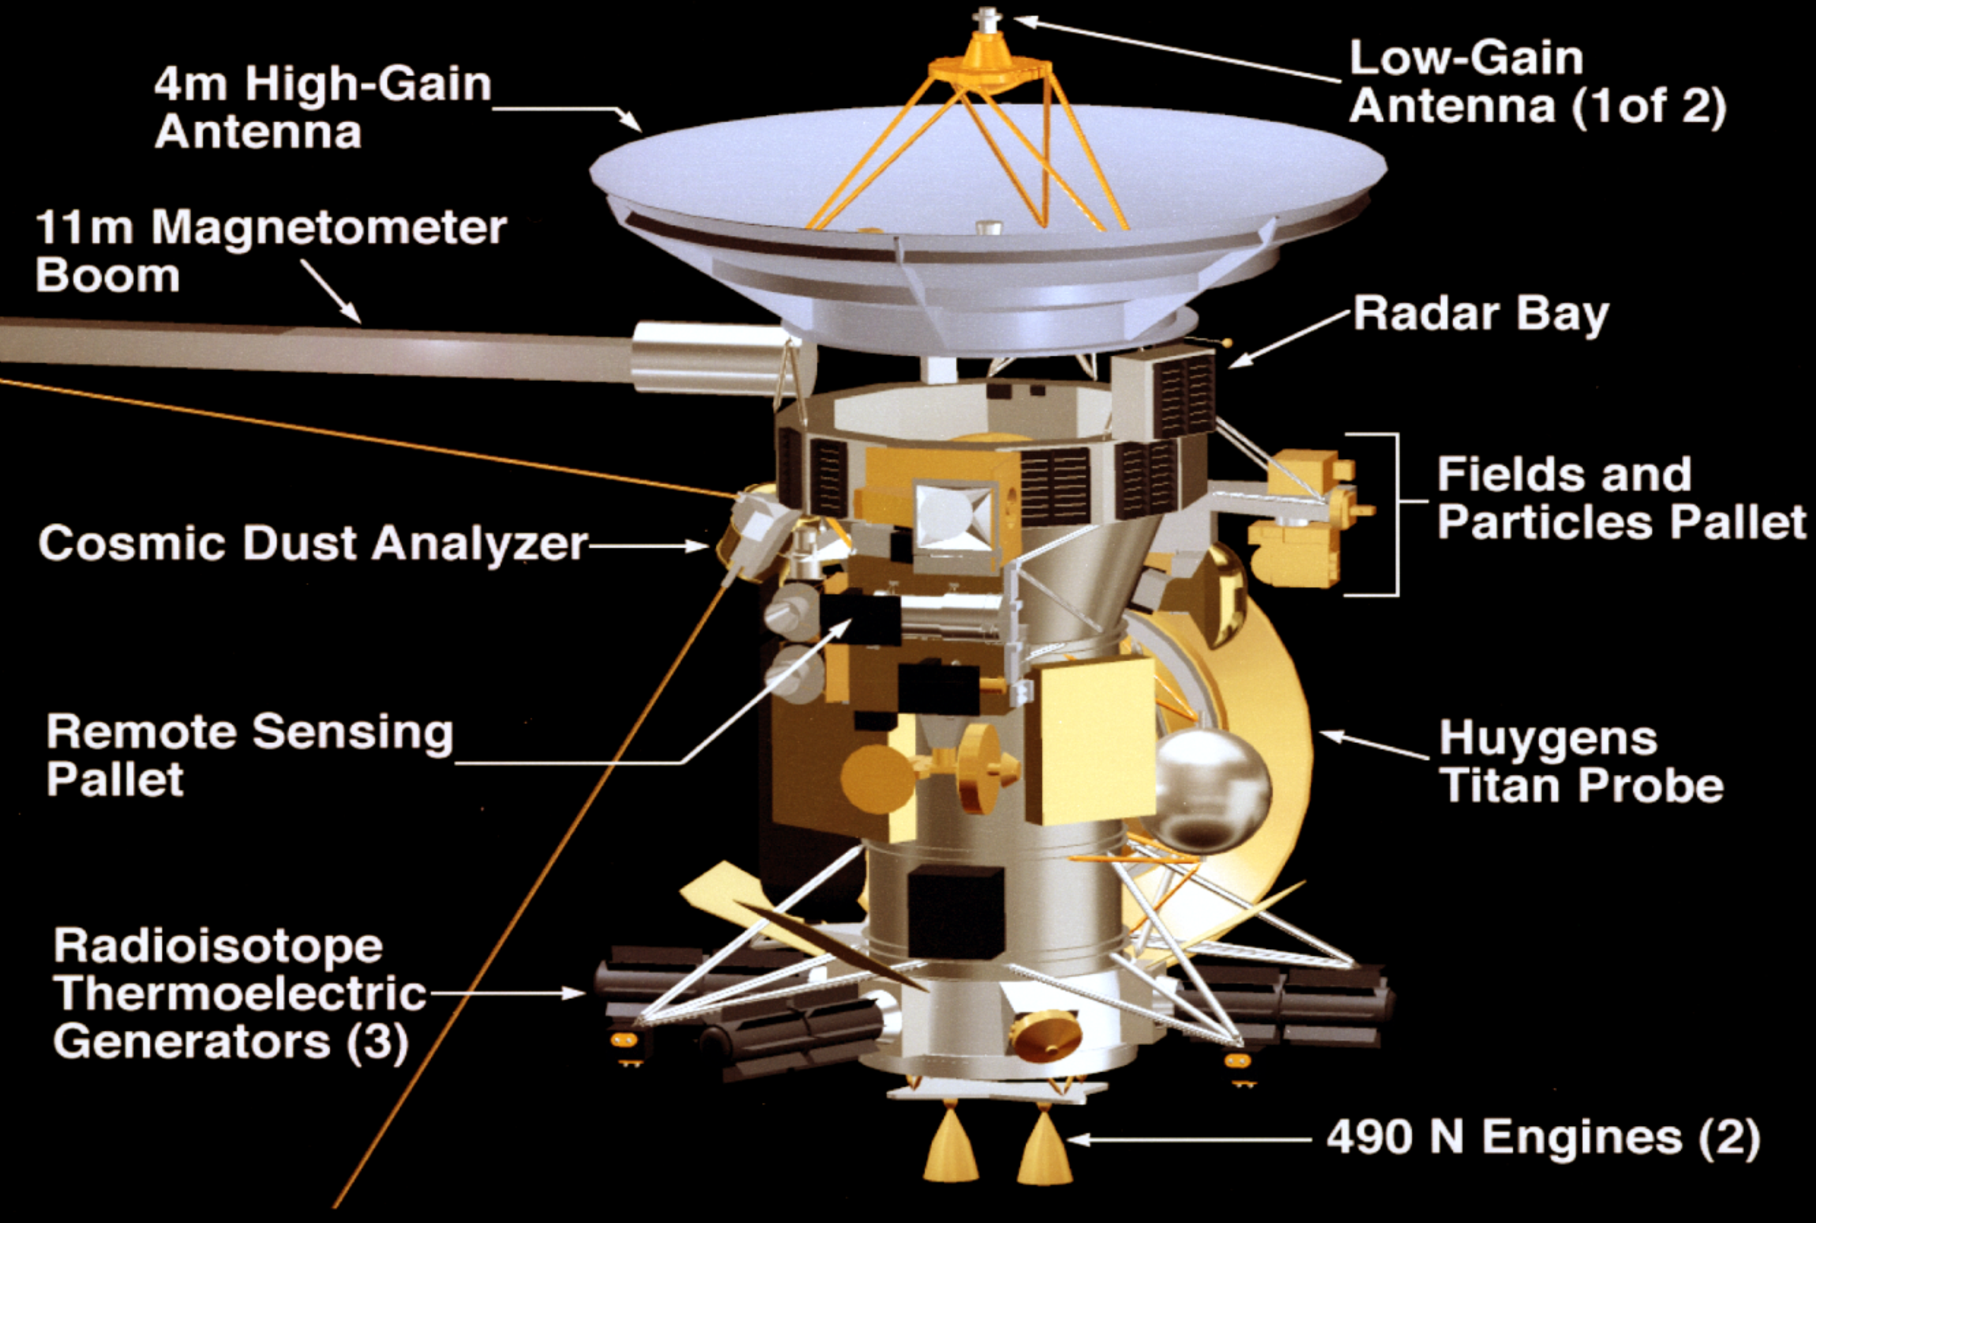
\includegraphics[width=1\textwidth]{cassini/spacecraft.pdf}
\caption[Diagram of the \textit{Cassini-Huygens} spacecraft]{Diagram of the \textit{Cassini-Huygens} spacecraft, from \citet{narvaez2004}. The spacecraft is about \SI{6.8}{m} in height.}
\label{cassini:fig:spacecraft}
\end{figure}

The \textit{Cassini-Huygens} mission (hereafter known as \textit{Cassini}) was a space mission designed to investigate the Saturn system, and was a collaboration between NASA, ESA and the Italian Space Agency (ASI). It was composed of a main \textit{Cassini} orbiter spacecraft with 12 instruments onboard, and the \textit{Huygens} probe with a further six, as described in \citet{matson2002}. A diagram of this spacecraft is shown in Figure~\ref{cassini:fig:spacecraft}. The instruments particularly relevant to the work in this thesis are discussed later in this chapter. 

Together, these instruments were designed such that the mission could investigate the entire Saturn system, from the interior of the planet itself to its atmosphere, rings, moons, and magnetosphere. The moon Titan was one of the key foci of the investigation, as it is the only moon in the solar system with a significant atmosphere, and it was initially thought to be a key source of plasma for the magnetosphere \citep{smith2004}. The \textit{Huygens} probe was therefore designed to detach from the main \textit{Cassini} orbiter and follow a single trajectory by parachute down to the surface of Titan, making \textit{in situ} measurements of Titan's atmosphere during the descent. The shield covering the \textit{Huygens} probe before it was deployed can be seen in Figure~\ref{cassini:fig:spacecraft}.

\section{Mission Timeline}\label{cassini:sec:timeline}
\textit{Cassini} launched from Cape Canaveral in Florida in October 1997, and finally arrived at the Saturn system in July 2004, after gravity-assist flybys of Venus, Earth and Jupiter. The mission was initially designed to operate for four years, from 2004-2008, and during this `Prime Mission' \textit{Cassini} completed 75 orbits of Saturn, and 44 flybys of Titan. The Prime Mission was incredibly successful, resulting in many exciting and unexpected discoveries about the Saturn system, such as the plumes of water being ejected from the icy moon Enceladus \citep{dougherty2006}. 

The mission was then extended by two years; the `Equinox Mission'. This extension allowed \textit{Cassini} to observe how the behaviour of the Saturn system changed with season, from northern winter to northern spring. (Saturn's obliquity relative to the ecliptic plane is \SI{26.7}{\degree}.) A Saturn year lasts 29 years, and the northern spring equinox occurred in August 2009, near the middle of the Equinox Mission. From a magnetospheric science perspective, equinox is a particularly interesting time to investigate the Saturn system, as the incident solar wind direction is parallel to Saturn's rotational/dipole equator, rather than at an angle slightly above or below. This means the solar wind conditions are approximately symmetrical in the northern and southern hemispheres, allowing for certain hemispheric effects, such as those discussed in Section~\ref{intro:sec:periodicities}, to be more readily investigated. Indeed, the data that are analysed in this thesis, particularly in Chapter~\ref{chap:equinox}, were acquired during \textit{Cassini's} Equinox Mission.

The mission was then further extended from 2010-2017, known as the `Solstice Mission', as the Saturn year continued into northern summer solstice in May 2017. The spacecraft trajectories were optimised to provide the most extensive coverage of scientifically interesting areas of the Saturn system, in the context of the entire mission. This culminated in the proximal orbits of the `Grand Finale', from April to September 2017. In each of these 22 final orbits, \textit{Cassini} traversed the gap between Saturn's atmosphere and the innermost ring, therefore orbiting far closer to the planet than at any other time in the mission, with a typical periapsis altitude of just ${\sim}\SI{2250}{km}$ above the 1-bar atmosphere level. This provided the opportunity to investigate scientific mysteries that still had not been answered from mission data so far, such as the core rotation rate of the planet and detailed internal magnetic field structure. The \textit{Cassini} mission then ended on 15 September 2017, as the spacecraft plunged into the planet's atmosphere and lost contact with Earth. The Grand Finale was designed in this way not just for maximum scientific reward, but also because the onboard rocket propellant used to manoeuvre the spacecraft was running out. With \textit{Cassini's} discovery of a likely sub-surface water ocean at Enceladus, and also prebiotic chemistry at Titan, the mission could not risk the spacecraft accidentally crashing into one of these moons and potentially contaminating them with Earth-based life forms. It was therefore necessary to deliberately impact the spacecraft into the planet Saturn itself.

\begin{figure}
\centering
\noindent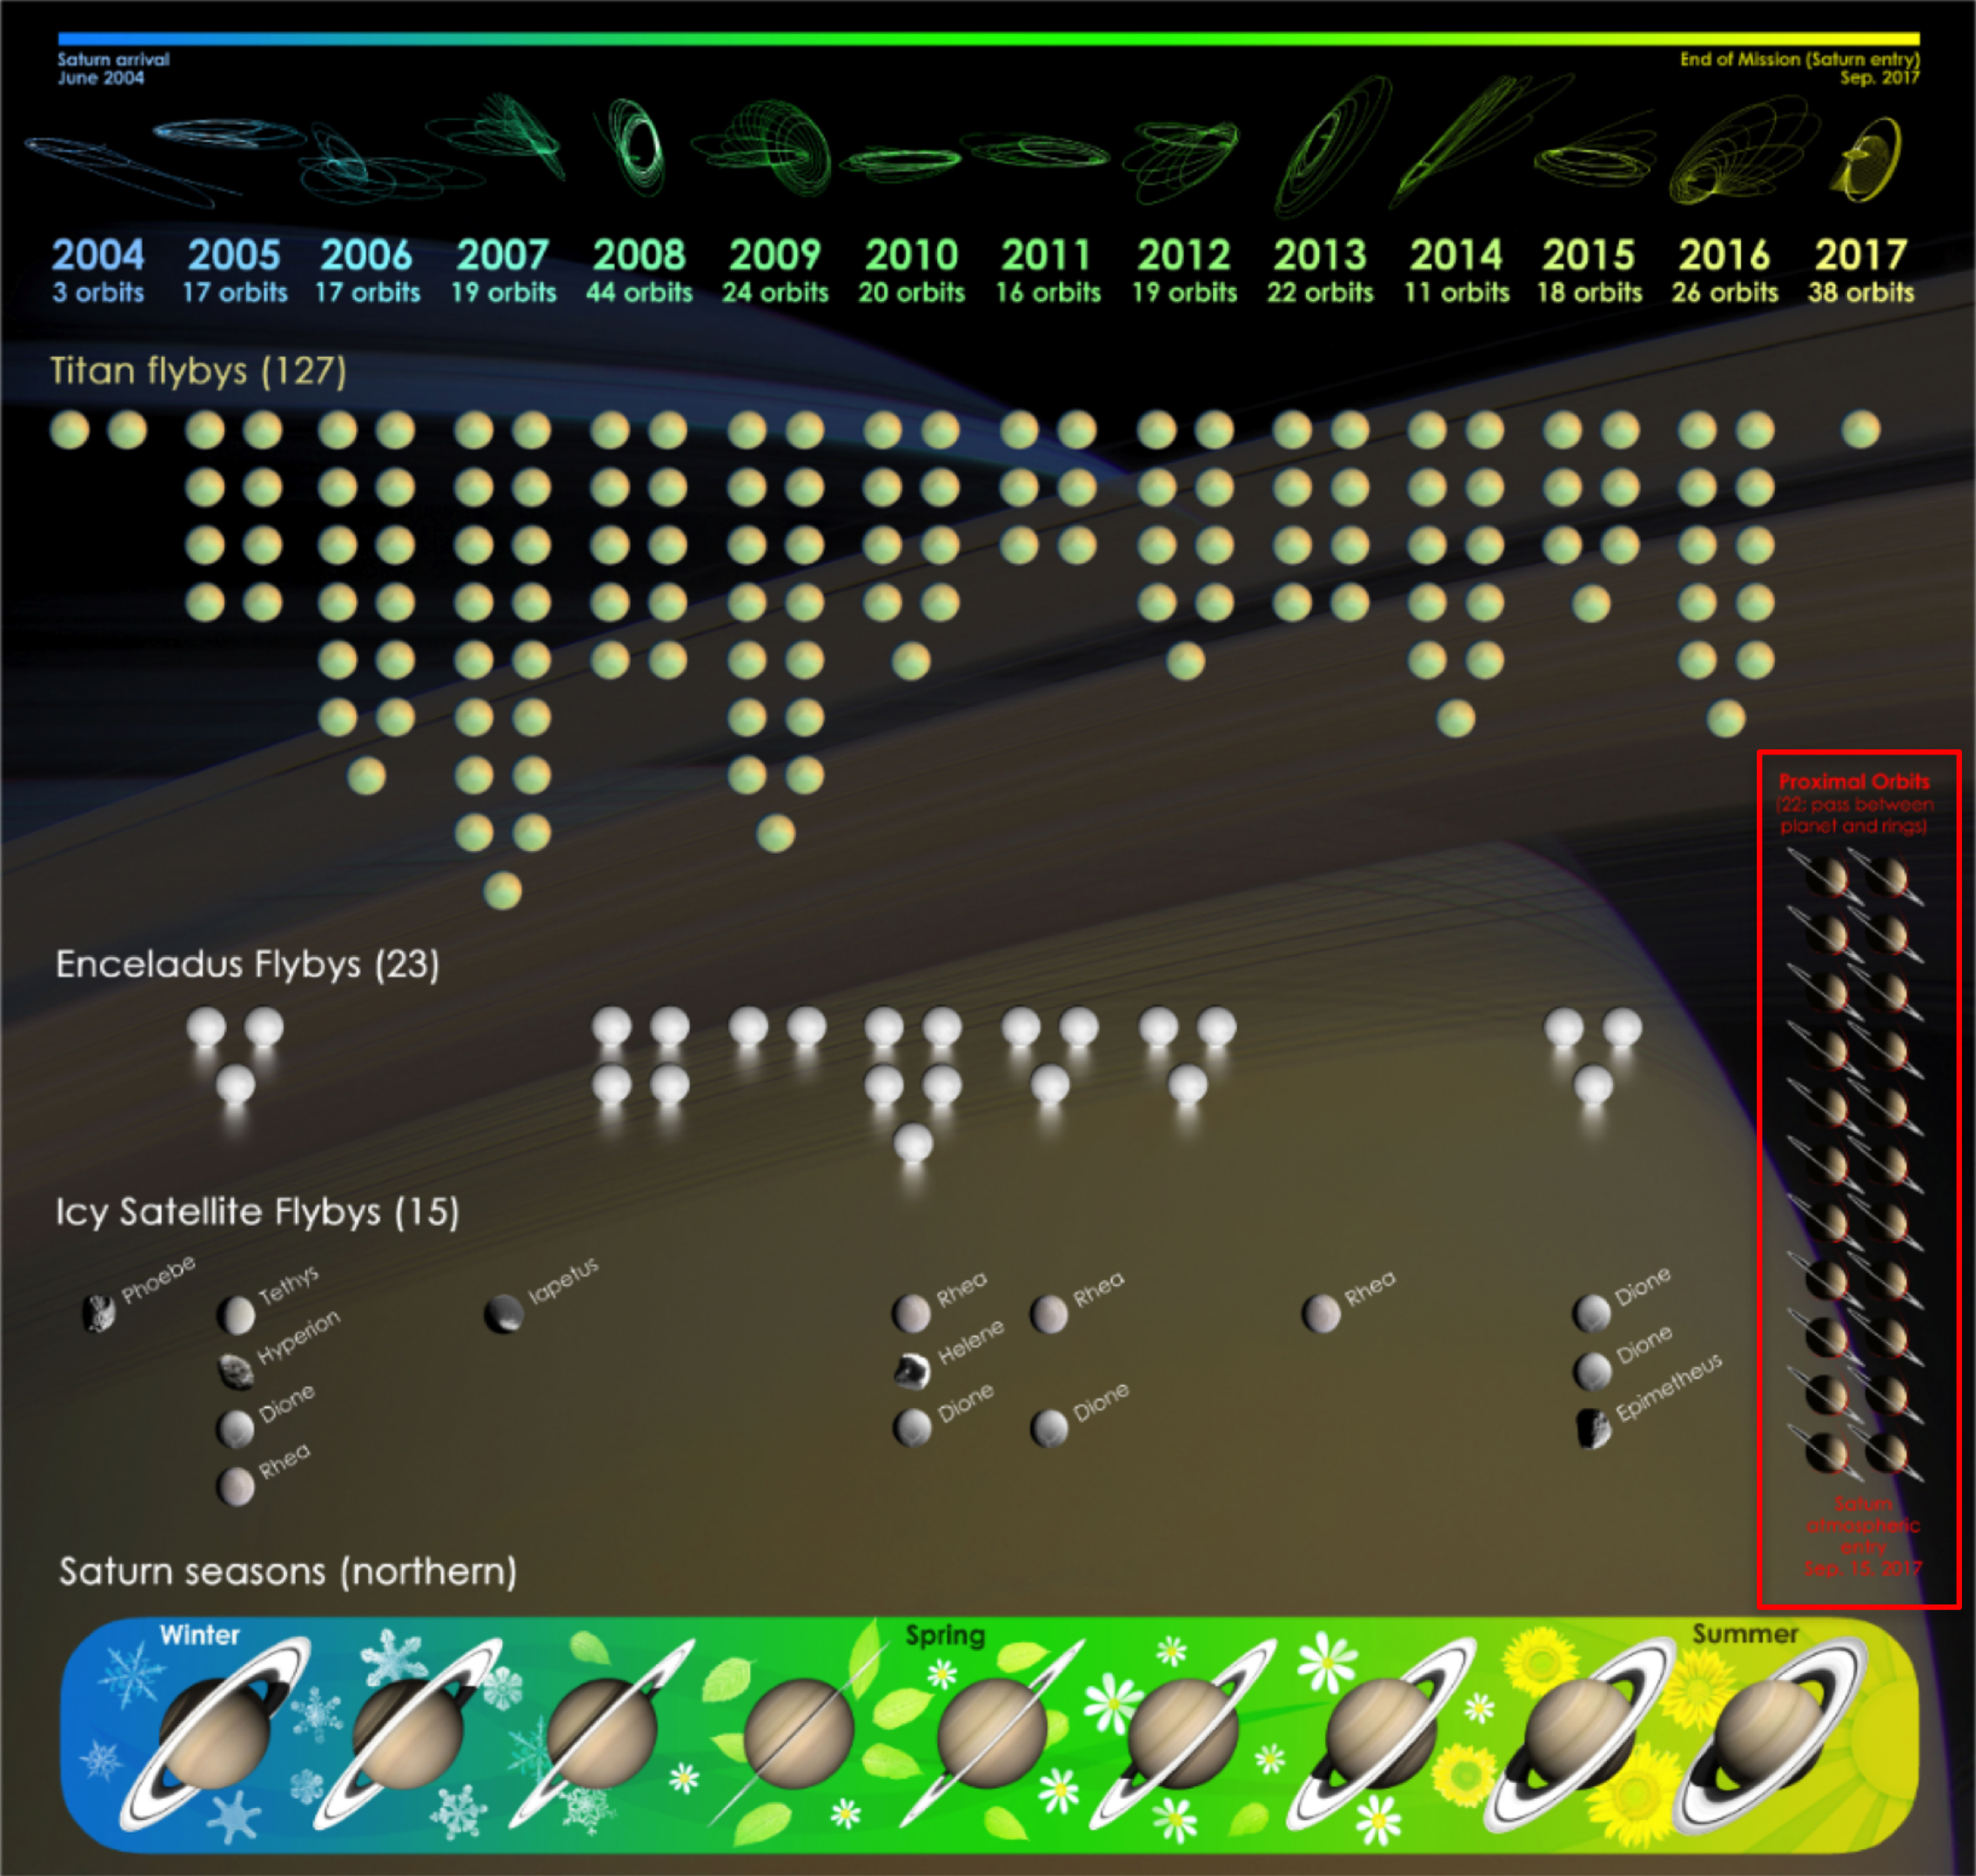
\includegraphics[width=0.9\textwidth]{cassini/mission_overview.jpg}
\caption[Diagram showing overview of \textit{Cassini }space mission.]{Diagram showing overview of \textit{Cassini} space mission orbit trajectories and moon flybys, from \citet{nasa2017}.}
\label{cassini:fig:missionoverview}
\end{figure}

Figure~\ref{cassini:fig:missionoverview} shows an overview of the entire \textit{Cassini} mission. At the top of the image the trajectories of the orbits are depicted, showing the extensive coverage \textit{Cassini} made in radial distance, latitude and local time. Also shown are the number of flybys of various moons, and  at the bottom the Saturn season is depicted. The proximal orbits, shown in red, are barely visible as they are so close to the Saturn surface.

\section{Key Instruments}
\subsection{Magnetometer (MAG)}
The dual technique magnetometer system (MAG) measured the magnitude and direction of Saturn's magnetic field \textit{in situ}, described in \citet{dougherty2004} and summarised here. The system was composed of a Vector/Scalar Helium Magnetometer (V/SHM), located at the end of the \SI{11}{m} long boom shown in Figure~\ref{cassini:fig:spacecraft}, and a FluxGate Magnetometer (FGM), located half way along it. This positioning was chosen so that measurements were contaminated as little as possible by magnetic fields generated by other instruments and electronics subsystems onboard the spacecraft itself, and also so that measurements from the two instruments could be compared for calibration. However the V/SHM malfunctioned early on in the mission, in November 2005, and so all the data presented in this thesis were measured solely by the FGM.

\begin{figure}
\centering
\noindent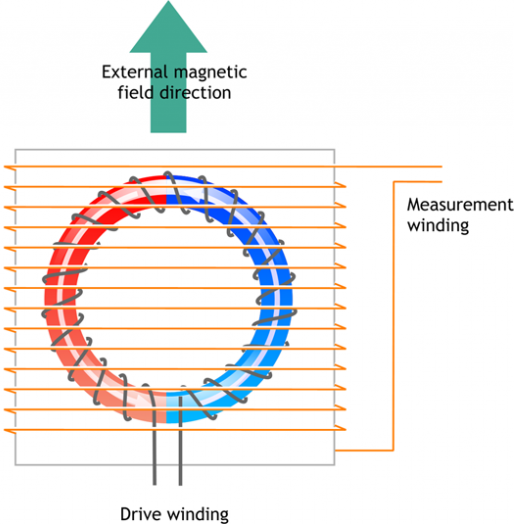
\includegraphics[width=0.6\textwidth]{cassini/FGMdiagram.png}
\caption[Diagram of how a fluxgate magnetometer works.]{Diagram showing basic construction of a fluxgate magnetometer, from \citet{carisma2018}. The drive winding and measurement winding are shown in dark grey and orange, respectively. The magnetic field induced in the core due to the current in  the drive winding  is shown by  the pale arrows on top of  the blue and red halves of the  core. The external magnetic field direction is shown by the large green arrow.}
\label{cassini:fig:FGMdiagram}
\end{figure}

The FGM was composed of three fluxgate sensors positioned orthogonally to each other, to measure the three vector components of the ambient magnetic field. A diagram showing the basic construction of one such sensor is shown in Figure~\ref{cassini:fig:FGMdiagram}. In each sensor, a coil of wire (`drive winding' in Figure~\ref{cassini:fig:FGMdiagram}) was wound around a high permeability ring-shaped core. A \SI{15.625}{\hertz} square wave current flowed through this drive coil, in order to induce a magnetic field in the core with clockwise orientation as shown by the pale arrows, until the core was saturated. Surrounding this entire set up was another coil of wire (`measurement winding' in Figure~\ref{cassini:fig:FGMdiagram}). In the absence of an external magnetic field, the two halves of the core shown in Figure~\ref{cassini:fig:FGMdiagram} would go into and out of saturation at the same time due to the drive winding current, and so there would  be no change of  flux through the measurement winding. However in the presence of an external magnetic field  oriented as shown by  the green arrow, one half of the core would become saturated more quickly than the other (depending on the phase of the drive winding current), causing a net change in magnetic flux through the measurement winding. In accordance with Faraday's law of  induction, this  would induce a voltage in  the measurement winding,  which could then be calibrated and used to measure the magnitude  of the external magnetic field. 

Only the component of the magnetic field perpendicular to the measurement winding orientation can be detected by this process, hence the need for three orthogonally positioned sensors. These three sensors were mounted on a single ceramic block, with the entire FGM  instrument  weighing just \SI{0.44}{kg}. The material ceramic was chosen for its low thermal expansion coefficient,  meaning  it changes shape very little under  changes in ambient temperature, and so any misalignment between the sensors was minimised.

The FGM had multiple operational ranges depending on the likely ambient magnetic field strength, which it could switch between automatically, and had a digital resolution of approximately one part in 10,000 depending on the range. The four ranges were $\pm\SI{40}{nT}$, $\pm\SI{400}{nT}$, $\pm\SI{10000}{nT}$, and $\pm\SI{44000}{nT}$, necessary for sampling different regions of Saturn's magnetosphere, where the magnetic  field strength  varies over many orders of magnitude. The normal downlink data rate for the FGM was $\SI{32}{vectors/s}$, although in this thesis we only investigate large-scale magnetospheric structures on large time scales, and so only present 1-hour-averaged MAG data. Such \textit{In situ} observations of Saturn's magnetic field revealed detailed information about the structure of Saturn's magnetosphere, such as the dynamical current sheet behaviour \citep[e.g.][]{provan2012}, and were also used to demonstrate the existence of an atmospheric plume at the icy moon Enceladus \citep{dougherty2006}. In Chapter~\ref{chap:equinox}, we use 1-hour-averaged MAG data measured near Saturn equinox in late 2009 to investigate the periodic flapping and breathing of Saturn's equatorial current sheet.

\subsection{Magnetospheric Imaging Instrument (MIMI)}
The Magnetospheric Imaging Instrument (MIMI) was a system for detecting both neutral and charged particles with high energies, described in \citet{krimigis2004} and summarised here. It was composed of three separate instruments, each described below.
\subsubsection{Ion and Neutral Camera (INCA)}
The Ion and Neutral Camera (INCA) was designed to detect both energetic neutral atoms (ENAs) and ion species over the range of energies $0.007{\--}\SI{3}{MeV/nucleon}$, and used time-of-flight information to determine the particle's energy and incident direction. A simple diagram of the instrument is shown in Figure~\ref{cassini:fig:INCAinstrument}.

\begin{figure}
\centering
\noindent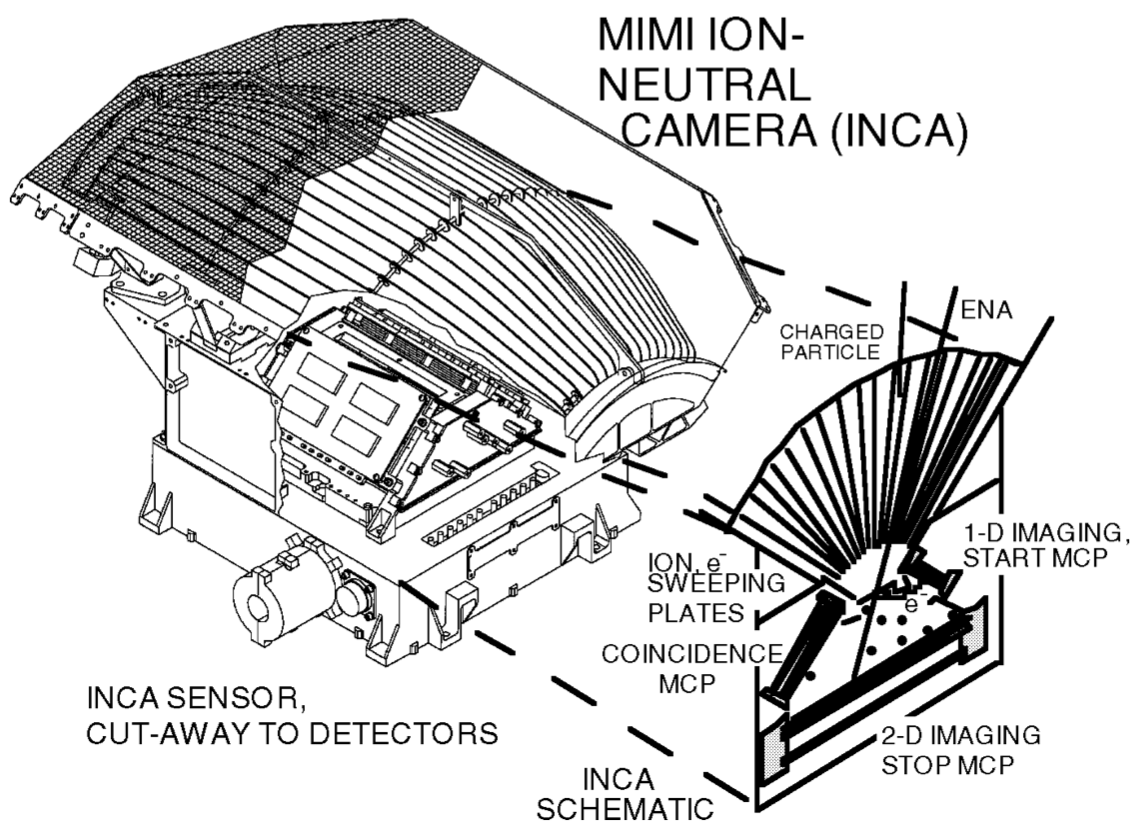
\includegraphics[width=0.8\textwidth]{cassini/INCAinstrument.png}
\caption[Diagram of the MIMI/INCA instrument.]{Cutaway diagram of the MIMI/INCA instrument, from \citet{krimigis2004}.}
\label{cassini:fig:INCAinstrument}
\end{figure}

Particles detected by the instrument would arrive broadly from above in the frame of  in Figure~\ref{cassini:fig:INCAinstrument}, and pass through the fan-like arrangement of serrated collimator plates, labelled as `ION, e- SWEEPING PLATES'. When in `neutral mode', these plates would be alternately charged at $\pm\SI{6}{kV}$ in order to sweep any energetic charged particles (with energies $\leq \SI{500}{keV}$) into the plate walls, thus excluding them from the internal detector. ENAs meanwhile would pass through the region unperturbed, and then penetrate a thin foil layer covering  the entrance slit. This would generate secondary electrons in the foil, which were steered to a 1-D microchannel plate (MCP) labelled as `1-D IMAGING, START MCP' in  Figure~\ref{cassini:fig:INCAinstrument}, recording the entrance position of the ENA and start time of travel. As the ENA proceeded further to the back of the instrument, it would penetrate another thin foil layer and  encounter a 2-D microchannel plate, labelled `2-D IMAGING STOP MCP', recording the exit position (in 2-D) and the end time of travel. At the same time, secondary electrons generated in the second thin foil layer would be steered to the microchannel plate  labelled `COINCIDENCE MCP', enabling a comparison with  the detection of the other plate in order to reduce background measurement noise. From all this information, the energy, mass, and incident direction of the ENA could be deduced. In particular it was found that the number of electrons generated in the foil was proportional to the mass of  the incident particle, which enabled the species (e.g.\ oxygen or hydrogen) of the particle to be determined. 

When operating in `ion mode', the  charge on the sweeping plates would be switched to zero so that ions could enter, and the instrument would detect ion species in a similar way. Neutrals would still also be able to enter the instrument in this mode, but in general the neutral counts were much lower and so would be drowned out by the incident ions.

\begin{figure}
\centering
\noindent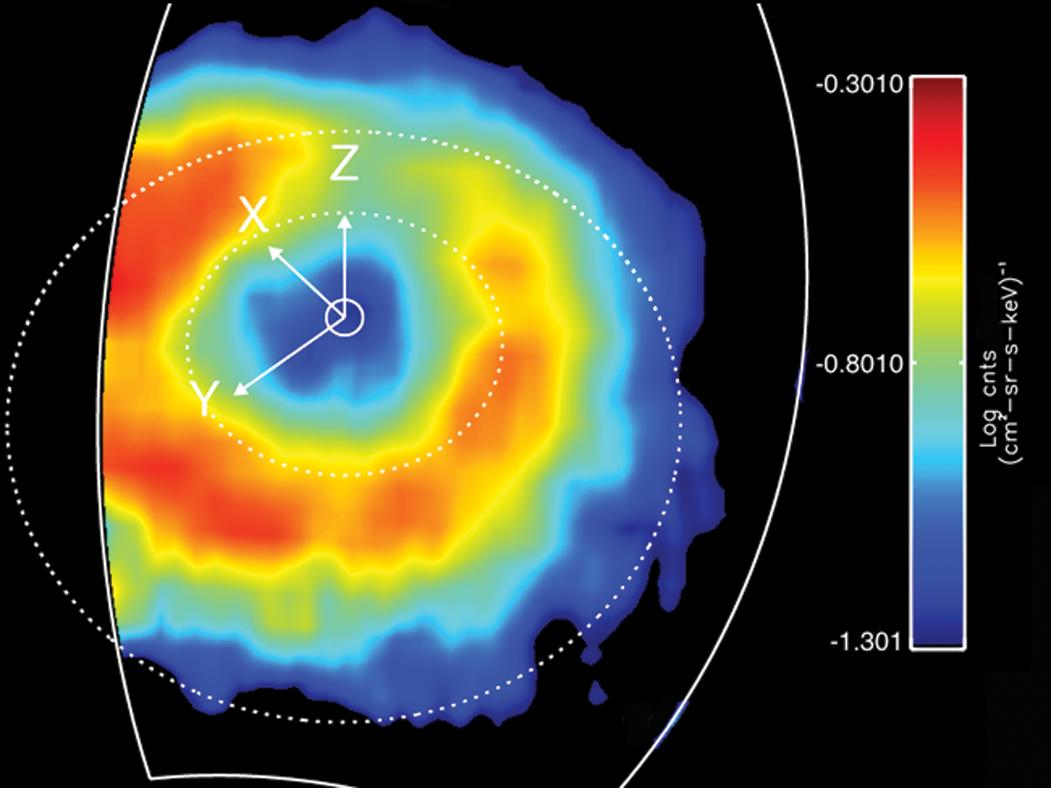
\includegraphics[width=0.8\textwidth]{cassini/INCAringcurrent.jpg}
\caption[ENA image of Saturn's ring current from MIMI/INCA.]{ENA image of Saturn's ring current from the MIMI/INCA instrument as viewed from a latitude of \SI{55}{\degree} above the northern hemisphere, averaged over a 3 hour period on 19 March 2007, from \citet{nasa2007}. Colour shows ENA intensity as per the colour bar. Saturn is at the  centre, and the white dashed lines show the orbits of the moons Rhea (\SI{8.7}{R_S}) and Titan (\SI{20.2}{R_S}). The Z axis points along Saturn's dipole/spin axis, the Y axis points approximately towards dusk, and the X axis points approximately  towards the Sun. The MIMI/INCA field of view is shown by the solid white line.}
\label{cassini:fig:INCAringcurrent}
\end{figure}

At Saturn, ENAs can be produced via charge exchange between singly-charged energetic ions and Saturn's neutral gas distribution (which originates from Saturn's rings and moons). Through collisions, an energetic ion can `steal' an electron from a neutral particle, such that the ion becomes neutral and is no longer constrained by the planetary magnetic field, and thus subsequently travels through space unperturbed. The energetic ions that make up Saturn's equatorial ring current can therefore be traced remotely via detection of ENAs originating from the equatorial plane. Figure~\ref{cassini:fig:INCAringcurrent} shows such an ENA image taken by \textit{Cassini's} MIMI/INCA instrument  on 19 March 2007, clearly showing the substantial ring current structure. 

\subsubsection{Charge-Energy-Mass Spectrometer (CHEMS)}
\begin{figure}
\centering
\noindent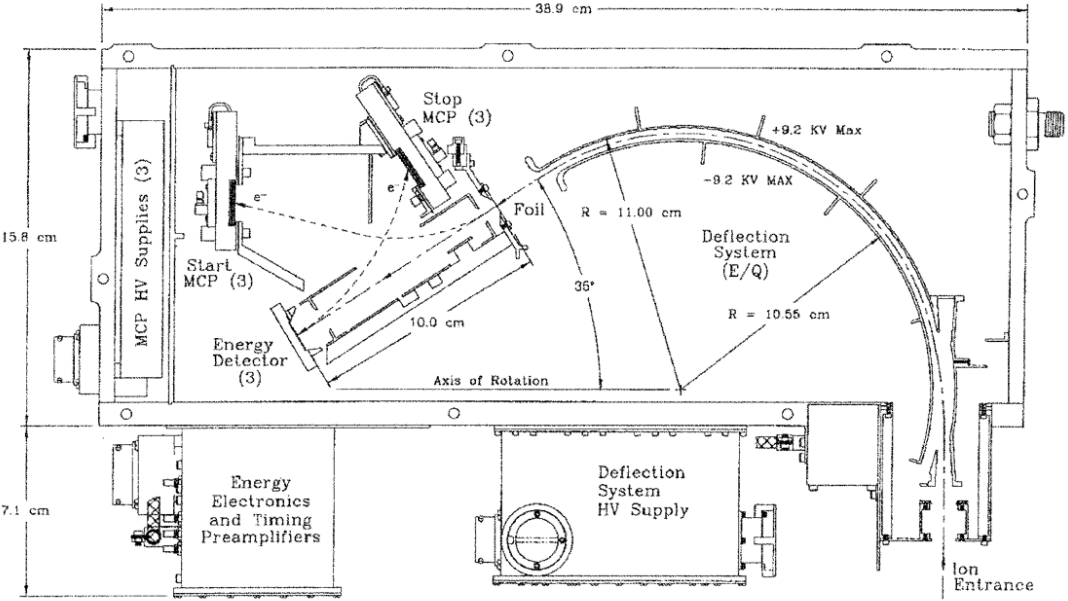
\includegraphics[width=0.9\textwidth]{cassini/CHEMSdiagram.png}
\caption[Diagram of the MIMI/CHEMS instrument.]{Diagram of the MIMI/CHEMS instrument, from \citet{krimigis2004}.}
\label{cassini:fig:CHEMSdiagram}
\end{figure}

The CHEMS instrument was designed to measure the charge, energy and mass of energetic ions, in the energy range $3{\--}\SI{220}{keV/e}$, using electrostatic deflection and time-of-flight information. The  instrument was mounted on \textit{Cassini} on the fields and particles pallet labelled in Figure~\ref{cassini:fig:spacecraft}. This positioning, combined  with the instrument construction described below, meant that during a spacecraft roll the instrument would have almost $4\pi$ steradian viewing geometry. This enabled the capability of measuring 3-D distribution functions of the energetic ion populations. A diagram of the instrument is shown in Figure~\ref{cassini:fig:CHEMSdiagram}.

As an ion entered the instrument from below in the frame on Figure~\ref{cassini:fig:CHEMSdiagram}, it would first encounter the `Deflection System', consisting of two oppositely charged spherical plates as shown in the diagram. The voltage across the plates was stepped through a series of logarithmically spaced  values over time to a maximum  of $\pm\SI{9.2}{keV}$, such that the plates acted as an energy per charge ($E/Q$) filter, allowing only ions within a small $E/Q$ band to pass through the system at any given time. If transmitted, the ion would then penetrate a thin foil layer, generating  secondary electrons that are then steered to the `Start MCP' microchannel plate, which would enable a start time-of-flight calculation to be made, as for MIMI/INCA. The ion would then impact the solid-state detector, labelled as `Energy Detector' in Figure~\ref{cassini:fig:CHEMSdiagram}, generating  secondary electrons that would then be steered to the `Stop MCP',  for the time-of-flight calculation. The solid-state detector also measured the residual energy of the incoming ion, so that the charge could be ascertained from the initial $E/Q$ measurement. Three independent telescopes with different viewing angles were included in CHEMS, hence the `(3)' labels at the energy detector, in order to enable the  aforementioned coverage of viewing geometry.

In combination with the other instruments that make up MIMI, MIMI/CHEMS was used to detect the widespread presence of energetic oxygen (O$^+$) and hydrogen (H$^+$) ions in Saturn's equatorial magnetosphere, and  to determine the partial pressures associated with the two populations \citep[e.g.][]{sergis2009}. The influence of his hot plasma population on the large-scale structure of the magnetosphere is discussed and investigated at length in this thesis, in particular in Chapters~\ref{chap:compress} and \ref{chap:LTsectors}.

\subsubsection{Low-Energy Magnetospheric Measurement System (LEMMS)}
\begin{figure}
\centering
\noindent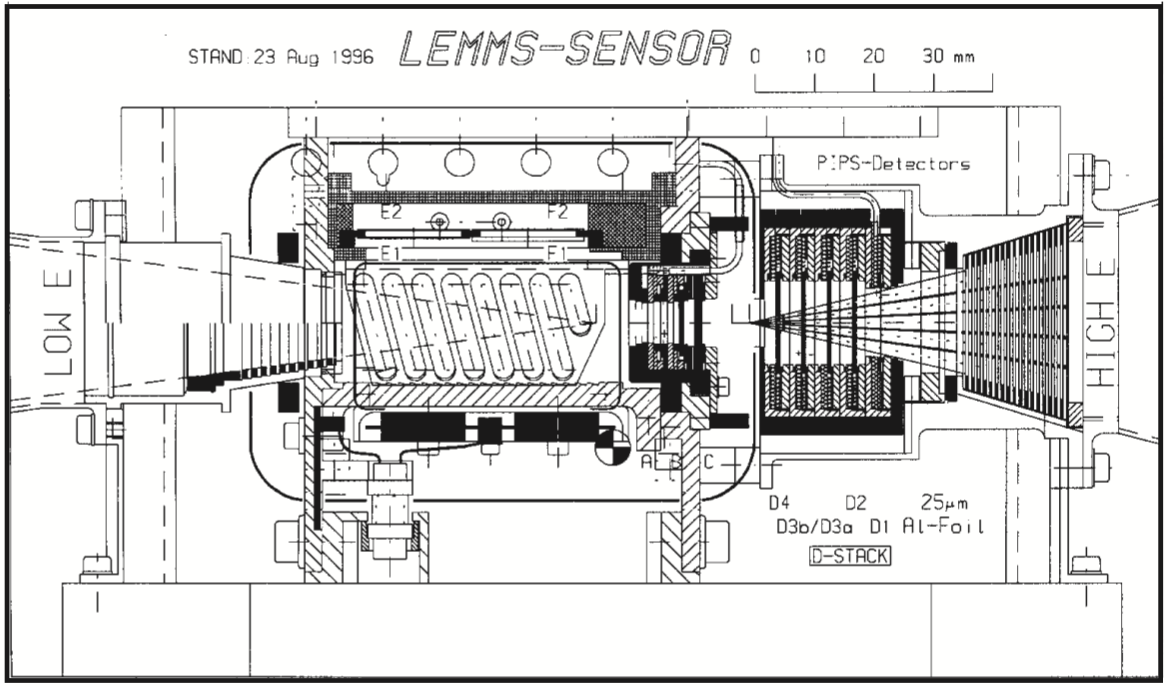
\includegraphics[width=0.9\textwidth]{cassini/LEMMSdiagram.png}
\caption[Diagram of the MIMI/LEMMS instrument.]{Diagram of the MIMI/LEMMS instrument, from \citet{krimigis2004}.}
\label{cassini:fig:LEMMSdiagram}
\end{figure}

The LEMMS instrument was designed to measure the distribution of energetic ion and electron fluxes. The instrument consisted of two oppositely oriented telescopes; a low-energy end, which measured ions with $E>\SI{30}{keV}$ and electrons with $E=\SI{15}{keV}{\--}\SI{1}{MeV}$, and a high-energy end, which measured ions with $E=1.5{\--}\SI{160}{MeV}$ and electrons with $E=0.1{\--}\SI{5}{MeV}$. The entire assembly was shielded with a platinum cover to avoid particles with energies $E<\SI{30}{MeV}$ penetrating the sides of the instrument. The instrument was mounted on a rotating platform to enable a larger total field of view; however, this mobility became compromised early on in the mission (early 2005), and so it remained in a fixed orientation with field of view closely aligned with one of the MIMI/CHEMS telescopes for the remainder of the mission. A diagram of the instrument is shown in Figure~\ref{cassini:fig:LEMMSdiagram}.

In the low-energy telescope (labelled `LOW E' on the left of Figure~\ref{cassini:fig:LEMMSdiagram}, an internal permanent magnet provided an inhomogeneous magnetic field, which separated the incoming ions and electrons that had passed into the instrument through the initial collimator. The electrons would be more strongly perturbed by the magnetic field than the ions, and so would be diverted to the semiconductor silicon detectors labelled E(1,2) and F(1,2), depending on their initial energies and incident directions. Incident ions, which are less strongly perturbed by in the presence of a magnetic field due to their higher mass (as discussed in this thesis, Section~\ref{intro:sec:singleparticle}), would proceed to the back of the instrument and strike the detectors labelled A and B. Data from the detectors could then be used to determine the energies of the incoming particles. 

In the high-energy telescope, a stack of detectors labelled D(1,2,3a,3b,4) detected incoming ions and electrons that had passed through the initial collimator on that side (plus a thin layer of aluminium foil, labelled `Al-Foil', included to prevent contamination from sunlight and lower energy ions). The combination of detections from the different detectors, which had different electronic thresholds, could then be used to distinguish ions and electrons. Between detectors B on the low-energy side and D4 on the high-energy side, a gold absorber labelled C was included to prevent lower energy ions penetrating through to the high-energy detectors.

Information from this instrument was used in combination with MIMI/CHEMS to characterise the distributions of the high energy plasma population in Saturn's magnetosphere, for example in \citet{sergis2017}. In Chapter~\ref{chap:LTsectors}, we use observations from this study in particular as inputs to the UCL/AGA magnetodisc model, in order to investigate how this hot plasma population influences magnetodisc structure at different local times.

\subsection{Plasma Spectrometer (CAPS)}
\begin{figure}
\centering
\noindent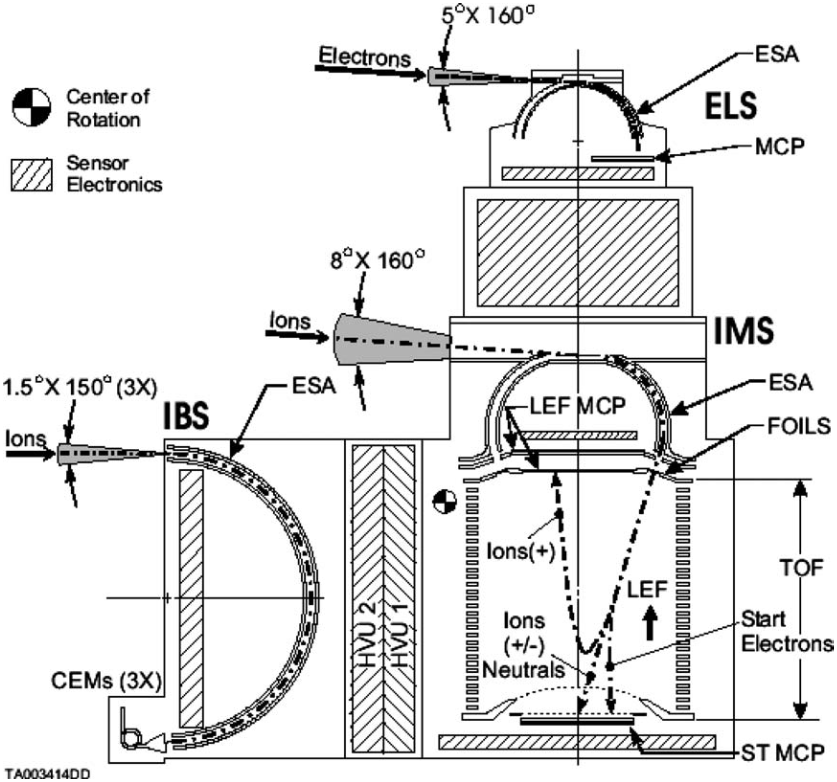
\includegraphics[width=0.8\textwidth]{cassini/CAPSdiagram.png}
\caption[Diagram of the CAPS instrument.]{Diagram of the CAPS instrument, from \citet{young2004}. The dot-dashed lines show the general shape of particle trajectories.}
\label{cassini:fig:CAPSdiagram}
\end{figure}

The CAPS instrument was used to measure the distributions of ions and electrons at lower energies than those observed by the MIMI instrument, and is described in \citet{young2004} and summarised here. It was made up of three separate sensors, including an electron spectrometer (ELS), ion mass spectrometer (IMS), and ion beam spectrometer (IBS), which is not discussed here as it was not used to make observations relevant to this thesis. ELS could detect electrons with energies in the range ${0.6}{-}\SI{29000}{eV}$, and IMS could detect ions in the range ${1}{-}\SI{50000}{eV}$. A diagram of the instrument is shown in Figure~\ref{cassini:fig:CAPSdiagram}. The entire instrument was mounted on a rotating platform on the underside of the `fields and particles pallet' shown in Figure~\ref{cassini:fig:spacecraft}, such that it had almost $2\pi$ steradians field of view, when not partially blocked by other parts of the spacecraft.

At both ELS and IMS, incoming particles first travelled between separated curved charged plates, labelled `ESA' (electrostatic analyser) in the diagram. As in the MIMI/CHEMS instrument, the voltage across the plates was stepped through a series of logarithmically spaced values over time, in order to filter only charged particles within a certain small range in $E/Q$ at a given time. 

For ELS, this corresponds to filtering for different energy electrons, as $Q$ is fixed for electrons. The angular distribution of the incoming electrons at each energy range was then determined based on where the electrons hit the microchannel plate, labelled `MCP' in Figure~\ref{cassini:fig:CAPSdiagram}. 

For IMS, the instrument performed time-of-flight calculations to determine the particle energies. The region labelled as `TOF' was charged at $\SI{-14.6}{kV}$ at the top, and $\SI{+14.6}{kV}$ at the bottom, generating a linear electric field labelled `LEF'. This would first accelerate ions that successfully exited the charged plates out through one of eight carbon foils, labelled `FOILS', generating secondary electrons to be steered to a microchannel plate to measure the start time of flight, as in the MIMI/INCA and CHEMS instruments. Positive ions with energies below ${\sim}\SI{15}{keV}$ would then be reflected back by the linear electric field into the `LEF MCP', while more energetic ions would be slowed down but still eventually penetrate the `straight-through' microchannel plate, labelled `ST MCP'. Molecular ions would break up on penetrating the initial carbon foils, but the resulting daughter products would still behave in this way and thus could be detected, and relevant information used to infer the original source particle. The peaks in the observed time-of-flight spectra would correspond to given ion mass-to-charge ratios $M/Q$, such that different ion species could then be identified.

Due to a technical fault, CAPS was switched off permanently in 2012. However, up until that time, observations made by the instrument were useful for investigating many magnetospheric phenomena at Saturn. Pertinent to this thesis, CAPS/ELS observations were used by \citet{pilkington2015} to identify instances when \textit{Cassini} crossed Saturn's magnetopause boundary, between the magnetosphere and the magnetosheath, as the sheath typically contains a more dense and lower energy population of electrons than the magnetosphere. This development of a database of crossings enabled a study of how the shape and size of the magnetopause surface varied under different conditions, and is complemented by the modelling study discussed in Chapter~\ref{chap:equinox}.

\added{Figure~\ref{cassini:fig:cassini_mp_crossing} shows data from both the MAG (top panel) and CAPS/ELS (bottom panel) instruments during a series of magnetopause crossings made by \textit{Cassini}, reproduced with permission from \citet{pilkington2015}. Crossings between the magnetosheath and magnetosphere are shown by the dashed magenta lines. In the CAPS/ELS data, a clear contrast can be seen between the low energy and high density (shown by the high electron count rate) electron population in the magnetosheath, and the high energy and low density electron population in the magnetosphere. In the MAG data, typically as the spacecraft crosses from the magnetosheath into the magnetosphere the total magnetic field strength  increases and becomes less variable, and there is also a rotation in the magnetic field components. More detail about identifying magnetopause crossings in this way can be found in \citet{pilkington2015}.}

\begin{figure}
\centering
\noindent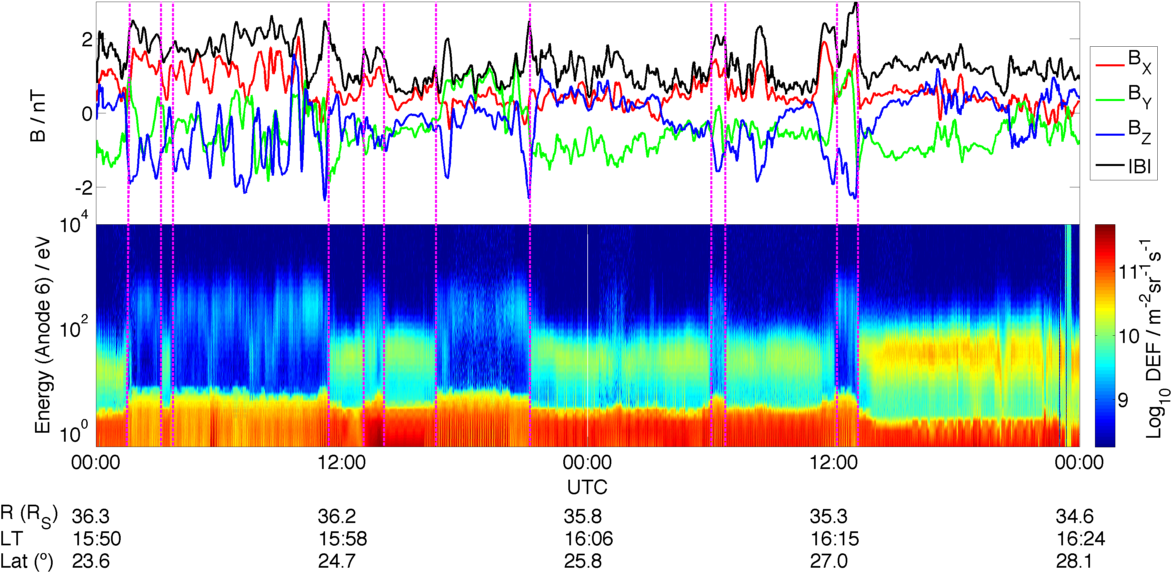
\includegraphics[width=0.8\textwidth]{cassini/els_DEF.png}
\caption[CAPS/ELS and MAG data during several magnetopause crossings.]{Several magnetopause crossings (dashed magenta lines) identified using \textit{Cassini} (top) MAG and (bottom) CAPS/ELS data, reproduced with permission from \citet{pilkington2015}. MAG data shown here has \SI{1}{\minute} resolution but has been smoothed using a moving average filter with a span of \SI{11}{\minute}. The radial distance, local time and latitude of the \textit{Cassini} spacecraft are given by the labels at the bottom of the figure.}
\label{cassini:fig:cassini_mp_crossing}
\end{figure}

\section{Summary}
The \textit{Cassini} space mission has, without a doubt, revolutionised our understanding of the large-scale structure and dynamics of Saturn's magnetosphere. Throughout this thesis, we refer to important results based on observations from the \textit{Cassini} instruments we have described herein. In addition, the \citet{achilleos2010a} model discussed in Section~\ref{intro:sec:forcebalancemodel} uses results from these instruments as equatorial boundary conditions. In the first study discussed in this thesis, we explore the influence of the variable hot plasma population detected by the MIMI instrument on the compressibility of Saturn's dayside magnetosphere.